\documentclass[12pt]{exam}
%\documentclass[answers, addpoints, 12pt,fleqn]{exam}

%\input{"C:/Users/Turk/Google Drive/LaTeX/header.tex"}
\usepackage{newcent}
\usepackage{lmodern}
\usepackage[T1]{fontenc}    % Ce package s'assure que les accents employés soient correctement affichés dans le fichier de sortie (.pdf ou .dvi).
\usepackage[utf8]{inputenc}    % latin1 permet l'utilisation des é,à,è,... directement, utf8 demande \'e, \`a , etc	
\usepackage[francais]{babel}
%\usepackage{icomma}
\usepackage{amsfonts,amsmath,amssymb,amsthm,mathrsfs}    %truc de maths, voir la doc   %thm permet de créer des environnement def,
\usepackage{multicol}       % plusieurs colonnes    http://www.ctan.org/pkg/multicol
\usepackage{graphicx,subfigure}
%\usepackage{fancybox}       % Box autour des # style Jayross http://www.ctan.org/pkg/fancybox
\usepackage{booktabs,multirow}       % Tables and stuff http://www.ctan.org/pkg/booktabs
\usepackage{xcolor}         % Texte en couleur
%\usepackage{titling}        % Donne accès à \thedate, qui affiche foo dans  la variable \date{foo}
%\usepackage{exercise}       %Permet d'inclure des exercices dans le texte
%\usepackage{mathtools}
\usepackage{MnSymbol}
\usepackage{gensymb}        %pour certains symboles
%%%%%%%%%%%%%%%%%%%%%%%%%%%%%%%%%%Commande pour valeurs absolues et normes
%\DeclarePairedDelimiter\abs{\lvert}{\rvert}%
%\DeclarePairedDelimiter\norm{\lVert}{\rVert}%

% Swap the definition of \abs* and \norm*, so that \abs
% and \norm resizes the size of the brackets, and the 
% starred version does not.
\makeatletter
\let\oldabs\abs
\def\abs{\@ifstar{\oldabs}{\oldabs*}}
%
\let\oldnorm\norm
\def\norm{\@ifstar{\oldnorm}{\oldnorm*}}
\makeatother
\usepackage{wasysym}
\newcommand{\hilight}[1]{\colorbox{yellow}{#1}}
%\renewcommand{\thesection}{\arabic{section}.}
\makeatletter
  \renewcommand\@seccntformat[1]{\csname the#1\endcsname.\quad}
\makeatother

\usepackage{float}
%\usepackage{enumitem}
\usepackage{enumerate}															%Permet de spécier apres \begin{enumerate}[]  comment décrire l'énumération (1) pour des nombres (a) (A) lettres, I des chiffre romains etc. {(a)}?
%\newlist{myitemize}{itemize}{10}
%\setlist[myitemize]{label=\textbullet}
%\newlist{myenumerate}{enumerate}{10}
%\setlist[myenumerate]{label=\arabic*.}
%\SetEnumitemKey{columns}{before=\begin{multicols}{#1},
%                         after=\end{multicols}}
\usepackage{ifpdf}
%\usepackage{pbox}   %Pour faire des saut de lignes dans les cellules d'un tableau
%\ifpdf
%   \usepackage{graphicx}
%   \usepackage{epstopdf}
%   \DeclareGraphicsRule{.eps}{pdf}{.pdf}{`epstopdf #1}                %Inclure des images EPS
%   \pdfcompresslevel=9
%\else
%   \usepackage{graphicx}
%\fi
\newcommand{\executeiffilenewer}[3]{%
\ifnum\pdfstrcmp{\pdffilemoddate{#1}}%
{\pdffilemoddate{#2}}>0%
{\immediate\write18{#3}}\fi%
} 

\setlength{\parindent}{1em}                       %Définie l'alinéa au début de chaque paragraphe


% Définit quelques commandes raccourcies
\newcommand{\Z}{\mathbb{Z}}                %Pour faire les Z,R,Q,N et C des ensembles plus rapidement
\newcommand{\R}{\mathbb{R}}
\newcommand{\Q}{\mathbb{Q}}
\newcommand{\N}{\mathbb{N}}
\newcommand{\C}{\mathbb{C}}
\newcommand{\D}{\mathbb{D}}
\newcommand{\Prob}[1]{\mathbb{P}\left(#1\right)}
\newcommand{\Probc}[2]{\mathbb{P}\left(#1~\left|\right .~#2\right)}
\newcommand{\E}[1]{\mathbb{E}\left(#1\right)}
\newcommand{\Ec}[2]{\mathbb{E}\left(#1~\left|\right .~#2\right)}
\newcommand{\indicator}[1]{1{\hskip -2.5 pt}\hbox{I}_{\left\{ {#1} \right\} }}
\newcommand{\pfrac}[2]{\left(\frac{#1}{#2}\right)}
\newcommand{\RH}{\overset{\text{\scalebox{0.8}{ R.H.}}}{=}}
\newcommand{\exbox}[1]{\vspace{10pt}%
\fbox{ \begin{minipage}{0.93\linewidth} \hfill\vspace{#1in} \end{minipage} }% 

\vspace{10pt}%
}
\DeclareMathOperator*{\argmin}{arg\,min}
\DeclareMathOperator*{\argmax}{arg\,max}
\DeclareMathOperator{\sech}{sech}
\DeclareMathOperator{\csch}{csch}
\DeclareMathOperator{\arcsec}{arcsec}
\DeclareMathOperator{\arccot}{arccot}
\DeclareMathOperator{\arccsc}{arccsc}
\DeclareMathOperator{\arccosh}{arccosh}
\DeclareMathOperator{\arcsinh}{arcsinh}
\DeclareMathOperator{\arctanh}{arctanh}
\DeclareMathOperator{\arcsech}{arcsech}
\DeclareMathOperator{\arccsch}{arccsch}
\DeclareMathOperator{\arccoth}{arccoth}
\DeclareMathOperator{\dom}{dom}  
\DeclareMathOperator{\Ima}{Im}       
\newcommand{\CQFD}{\begin{flushright}   %pour faire un carré de cqfd (blanc) ou CCQFD (noir)
$\blacksquare$	
\end{flushright}}
\newcommand{\cqfd}{\begin{flushright}
$\Box$	
\end{flushright}}
\usepackage{layout}    %Permet d'afficher le layout du texte, pour voir les marges etc. Utiliser \layout quelque part dans le texte
\linespread{1.1}																					%interligne
\allowdisplaybreaks[1]          %Évite les grands espaces verticaux en allouant un align, align* à s'étendre sur plusieurs pages
\theoremstyle{definition}       %  Style pour les \newtheorem, choix entre plain--definition--remark, possibilité de faire custom, voir ci-dessous
%\newtheorem{corollary}{Corollaire}[section]
%\newtheorem{definition}{Définition}[section]
%\newtheorem{example}{Exemple}[section]
%\newtheorem{lemma}{Lemme}[section]
%\newtheorem{proposition}{Proposition}[section]
%\newtheorem{remark}{Remarque}[section]
%\newtheorem{theorem}{Théorème}[section]


% Si vous préférez que les corollaires, definitions, théorèmes, etc. soient numérotés par le même compteur, utilisez plutôt ce bloc de commandes: 

\newtheorem{corollary}{Corollaire}[section]
\newtheorem{definition}[corollary]{Définition}
\newtheorem{example}[corollary]{Exemple}
\newtheorem{lemma}[corollary]{Lemme}
\newtheorem{proposition}[corollary]{Proposition}
\newtheorem{remark}[corollary]{Remarque}
\newtheorem{theorem}[corollary]{Théorème}
\newtheorem*{theorem*}{Théorème}
%%%%%%%%%%%%%%%%%%%%%%%%%%%%%%%%%%%%%%%%%%%%%%%%%%%%%%%
%%%%%%%%%%%%%%%%%%%%%%%%%%%%%%%%%%%%%%%%%%%%%%%%%%%%%%%
% Création d'une commande permettant de zoomer sur une partie du PDF  \zoombox[linewidth]{object}   \startzoom[linewidth]{label} \stomzoom{label} aussi en mode *
%  Voir http://tex.stackexchange.com/questions/12290/automatic-zoom-in-hypertext-boxes-in-pdf/12293#12293
\makeatletter
\newsavebox\zb@x
\newcounter{z@@m}
\usepackage{calc}
\newdimen\B@r\newdimen\P@r
\newdimen\@zw\newdimen\@zh\newdimen\@zd

\newcommand{\zoombox}[2][0]{%
  \leavevmode%
  \sbox\zb@x{#2}%
  \setlength\B@r{1pt*\ratio{\wd\zb@x}{\ht\zb@x+\dp\zb@x}}%
  \setlength\P@r{1pt*\ratio{\paperwidth}{\paperheight}}%
  \ifdim\B@r>\P@r\relax%
    \setlength\@zw{\wd\zb@x}\setlength\@zh{\@zw*\ratio{\paperheight}{\paperwidth}}%
    \setlength\@zd{(\@zh-\ht\zb@x-\dp\zb@x)*\real{0.5}+\dp\zb@x}%
    \setlength\@zh{\@zh-\@zd}%
  \else%
    \setlength\@zh{\ht\zb@x+\dp\zb@x}%
    \setlength\@zw{\@zh*\ratio{\paperwidth}{\paperheight}}%
    \setlength\@zh{\ht\zb@x}\setlength\@zd{\dp\zb@x}%
  \fi%
  \makebox[0pt][l]{\makebox[\wd\zb@x][c]{\makebox[\@zw][l]{%
    \pdfdest name {zbfs\thez@@m} fitr
      width  \@zw\space
      height \@zh\space
      depth  \@zd\space
  }}}%
  \pdfdest name {zb\thez@@m} fitr
    width  \wd\zb@x\space
    height \ht\zb@x\space
    depth  \dp\zb@x\space
  \immediate\pdfannot 
    width  \wd\zb@x\space
    height \ht\zb@x\space
    depth  \dp\zb@x\space
  {%
    /Subtype/Link/H/N
		/C [\@linkbordercolor]
    /Border [0 0 #1 [1 2]]
    /A <<
      /S/JavaScript
      /JS (
        if(typeof(zoomed)=='undefined'||!zoomed){
          var lastView=this.viewState;
          if(app.fs.isFullScreen) this.gotoNamedDest('zbfs\thez@@m');
          else this.gotoNamedDest('zb\thez@@m');
          zoomed=true;
        }else{
          this.viewState=lastView;
          zoomed=false;
        }
      )
    >>
  }%
  \usebox{\zb@x}%
  \stepcounter{z@@m}%
}   
\makeatother
%%%%%%%%%%%%%%%%%%%%%%%%%%%%%%%%%%%%%%%%%%%%%%%%%%%%%%%%%%%%%%%%%%%%%%%%%%%%%%%%%%%%%%%%%%%%%%%%%%%%%%%%%%%%%%%%%%%%%%%
\makeatletter
\InputIfFileExists{\jobname.zom}{}{}                                                                         
\newwrite\zoomdat
\immediate\openout\zoomdat=\jobname.zom                                                                      
\newcommand{\startzoombox}[2][0]{%                                                                           
  \leavevmode%                                                                                               
  \pdfsavepos%
  \protected@write\zoomdat{}{%
  \string\expandafter\string\def\string\csname\space zb#2.ulx\string\endcsname{%                             
    \noexpand\number\pdflastxpos}%
  \string\expandafter\string\def\string\csname\space zb#2.uly\string\endcsname{%                             
    \noexpand\number\pdflastypos}%                                                                           
  }%
  \ifcsname zb#2.ulx\endcsname\ifcsname zb#2.lrx\endcsname%
    \edef\zoomwd{\dimexpr \csname zb#2.lrx\endcsname sp- \csname zb#2.ulx\endcsname sp\relax}%               
    \edef\zoomdp{\dimexpr \csname zb#2.uly\endcsname sp- \csname zb#2.lry\endcsname sp\relax}%               
    \pdfdest name {zb#2.in} fitr                                                                             
      width \zoomwd                                                                                          
      height 0pt
      depth \zoomdp
    \immediate\pdfannot                                                                                      
      width \zoomwd                                                                                          
      height 0pt
      depth \zoomdp                                                                                          
    {%
      /Subtype/Link/H/N 
      /Border [0 0 1 [1 2]]                                                                                  
      /A <<
        /S/JavaScript                                                                                        
        /JS (
          if(typeof(zoomed)=='undefined'||!zoomed){                                                          
            var lastView=this.viewState;                                                                     
            zoomed=true;
            this.gotoNamedDest('zb#2.in');                                                                   
          }else{
            this.viewState=lastView;                                                                         
            zoomed=false;                                                                                    
          }                                                                                                  
        )                                                                                                    
      >>                                                                                                     
    }%
  \fi\fi%                                                                                                    
}
\def\stopzoombox#1{%\leavevmode%                                                                             
  \leavevmode%                                                                                               
  \pdfsavepos%
  \protected@write\zoomdat{}{%
  \string\expandafter\string\def\string\csname\space zb#1.lrx\string\endcsname{%                             
    \noexpand\number\pdflastxpos}%
  \string\expandafter\string\def\string\csname\space zb#1.lry\string\endcsname{%                             
    \noexpand\number\pdflastypos}%                                                                           
  }%                                                                                                         
}
\def\startzoom{%
  \@ifstar\@startzoomstar\@startzoom%                                                                        
}
\newcommand{\@startzoom}[2][0]{%
  \raisebox{\baselineskip}[0pt][0pt]{\startzoombox[#1]{#2}}%                                                 
}
\newcommand{\@startzoomstar}[2][0]{%
  \makebox[0pt][r]{\raisebox{\baselineskip}[0pt][0pt]{\startzoombox[#1]{#2}}%                                
  \hspace{\parindent}}%                                                                                      
}
\def\stopzoom{%
  \@ifstar\@stopzoomstar\@stopzoom%                                                                          
}
\def\@stopzoom#1{%
  \raisebox{-1ex}[0pt][0pt]{\stopzoombox{#1}}%                                                               
}
\def\@stopzoomstar#1{%
  \hfill\raisebox{-1ex}[0pt][0pt]{\stopzoombox{#1}}%                                                         
}
\makeatother
%%%%%%%%%%%%%%%%%%%%%%%%%%%%%%%%%%%%%%%%%%%%%%%%%%%%%%%%%%%%%%%%%%%%%%%%%%%%%%%%%%%%%%%%%%%%%%%%%%%%%%%
\usepackage{hyperref}    %  Doit être en dernier, ou presque
\hypersetup{
%SS-option        %Défaut    %effet
%anchorcolor       %black     %set color of anchors
%backref 		      %false     %do bibliographical back references
%baseurl           %empty     %set base URL for document
%bookmarks         %true      %make bookmarks
%bookmarksnumbered %false     %put section numbers in bookmarks
%bookmarksopen     %false     %open up bookmark tree
%bookmarksopenlevel%\maxdimen %level to which bookmarks are open
%bookmarkstype     %toc       %to specify which ‘toc’ file to mimic
%breaklinks        %false     %allow links to break over lines
%CJKbookmarks      %false     %to produce CJK bookmarks
%citebordercolor   %0 1 0     %color of border around cites
%citecolor         %green     %color of citation links
%colorlinks        %false     %color links
                   %true      %(tex4ht, dviwindo)
%debug             %false     %provide details of anchors defined; same as verbose
%destlabel         %false     %destinations are named by the first \label after the anchor creation
%draft             %false     %do not do any hyperlinking
%dvipdfm                      %use dvipdfm backend
%dvipdfmx                     %use dvipdfmx backend
%dvips                        %use dvips backend
%dvipsone                     % use dvipsone backend
%dviwindo                     %use dviwindo backend
%encap                        %to set encap character for hyperindex
%extension                    %dvi suffix of linked files
%filebordercolor  %0 .5 .5    %color of border around file links
%filecolor        %cyan       %color of file links
%final            %true       %opposite of option draft
frenchlinks=true,      %false      %use small caps instead of color for links
%hyperfigures     %false      %make figures hyper links
%hyperfootnotes   %true       %set up hyperlinked footnotes
%hyperindex       %true       %set up hyperlinked indices
%hypertex                     %use HyperTEX backend
%hypertexnames    %true       %use guessable names for links
%implicit         %true       %redefine LATEX internals
%latex2html                   %use LATEX2HTML backend
linkbordercolor={0 0 1},  %1 0 0      %color of border around links
linkcolor=blue,       %red        %color of links
%linktocpage      %false      %make page number, not text, be link on TOC, LOF and LOT
%menubordercolor  %1 0 0      %color of border around menu links
%menucolor        %red        %color for menu links
%nativepdf        %false      %an alias for dvips
%naturalnames     %false      %use LATEX-computed names for links
%nesting          %false      %allow nesting of links
%pageanchor       %true       %put an anchor on every page
%pagebackref      %false      %backreference by page number
pdfauthor=Yasmine Tawfik,        %empty      %text for PDF Author field
%pdfborder        %0 0 1      %width of PDF link border
                  %0 0 0      %(colorlinks)
%pdfcenterwindow  %false      %position the document window in the center of the screen
%pdfcreator       %LaTeX with %text for PDF Creator field
								  %hyperref
								  %package
%pdfdirection     %empty      %direction setting
pdfdisplaydoctitle=true, % false    %display document title instead of file name in title bar
%pdfduplex        %empty      %paper handling option for print dialog
%pdffitwindow     %false      %resize document window to fit document size
%pdfhighlight     %/I         %set highlighting of PDF links
%pdfinfo          %empty      % alternative interface for setting document information
%pdfkeywords      %empty      %text for PDF Keywords field
%pdflang          %relax      %PDF language identifier (RFC 3066)
%pdfmark          %false      %an alias for dvips
%pdfmenubar       %true       %make PDF viewer’s menu bar visible
%pdfnewwindow     %false      %make links that open another PDF file start a new window
%pdfnonfullscreenpagemode %empty        %page mode setting on exiting full-screen mode
%pdfnumcopies             %empty        %number of printed copies
%pdfpagelayout            %empty        %set layout of PDF pages
%pdfpagemode              %empty        %set default mode of PDF display
%pdfpagelabels            %true         %set PDF page labels
%pdfpagescrop             %empty        %set crop size of PDF document
%pdfpagetransition        %empty        %set PDF page transition style
%pdfpicktraybypdfsize     %empty       %set option for print dialog
%pdfprintarea             %empty       %set /PrintArea of viewer preferences
%pdfprintclip             %empty       %set /PrintClip of viewer preferences
%pdfprintpagerange        %empty       %set /PrintPageRange of viewer preferences
%pdfprintscaling          %empty       %page scaling option for print dialog
%pdfproducer              %empty       %text for PDF Producer field
%pdfremotestartview        %Fit         %starting view of remote PDF documents
%pdfstartpage             %1           %page at which PDF document opens
%pdfstartview             %Fit         %starting view of PDF document
pdfsubject=Mathématiques,               %empty       %text for PDF Subject field
%pdftex                                % use pdfTEX backend
%pdftitle                 %empty       %text for PDF Title field
%pdftoolbar               %true        %make PDF toolbar visible
%pdftrapped               %empty       %Sets the document information Trapped entry. Possible values are True, False and Unknown. An empty value means, the entry is not set.
%pdfview                  %XYZ         %PDF ‘view’ when on link traversal
%pdfviewarea              %empty       %set /ViewArea of viewer preferences
%pdfviewclip              %empty       %set /ViewClip of viewer preferences
%pdfwindowui              %true        %make PDF user interface elements visible
%plainpages               %false       %do page number anchors as plain Arabic
%ps2pdf                                %use ps2pdf backend
%raiselinks               %false       %raise up links (for HyperTEX backend)
%runbordercolor           %0 .7 .7     %color of border around ‘run’ links
%runcolor                 %filecolor   %color of ‘run’ links
%setpagesize              %true        %set page size by special driver commands
%tex4ht                                %use TEX4ht backend
%textures                              %use Textures backend
%unicode                  %false       %Unicode encoded pdf strings
%urlbordercolor           %0 1 1       %color of border around URL links
%urlcolor                 %magenta     %color of URL links
%verbose                  %false       %be chatty
%vtex                                  %use VTeX backend
%xetex                                 %use XeTEX backend
}
\usepackage[all]{hypcap}        % needed to help hyperlinks direct correctly, load after hyperref
\pagestyle{headandfoot}
\usepackage{afterpage}
\newcommand\blankpage{%
    \null
    \thispagestyle{empty}%
    \addtocounter{page}{-1}%
    \newpage}
\firstpageheadrule
\firstpageheader{Méthodes quantitatives en sciences humaines - 360-300-RE}{}{Formatif 1}                              %exam class
\firstpagefooter{}{}{\thepage}
\firstpagefootrule
\runningheadrule
\runningheader{Méthodes quantitatives en sciences humaines - 360-300-RE}{}{Formatif 1}  
\runningfooter{YT}{}{\thepage}
\runningfootrule
\CorrectChoiceEmphasis{\color{blue}\itshape}
\SolutionEmphasis{\color{blue}\itshape}
\checkboxchar{$\Box$}
\checkedchar{$\blacksquare$}
\qformat{\textbf{Question \thequestion:} \hfill}    %Pour un exam
%\qformat{\shadowbox{\textbf{Exercice} \thequestion}  \hfill}           %Pour un exercice
%\renewcommand{\questionlabel}{$\shadowbox{\thequestion}$}            % Liste à la Jérémie

%%%%%%%%%%%%%%%%%%%%%%
%%%Titre du document%%
%%%%%%%%%%%%%%%%%%%%%%
\title{Formatif examen 1}

\author{Yasmine Tawfik - Cégep Gérald-Godin}
\date{Hiver $2022$}

%\begin{document}
%\maketitle
%\thispagestyle{headandfoot}
%\printanswers    %Commente cette ligne pour ne pas afficher les solutions
%\begin{center}
%\fbox{\fbox{\parbox{5.5in}{\centering
%\emph{Consignes:} Répondez aux questions suivantes individuellement.}}} %Si vous manquez d'espace, vous pouvez utiliser le dos en indiquant \textbf{clairement} le numéro de la question que vous faites}}}
%\end{center}
%\vspace{0.1in}
%\makebox[\textwidth]{Nom:\enspace\hrulefill}
%\makebox[\textwidth]{Cours:\enspace\hrulefill}
%\vspace{0.2in}


\usepackage[margin=2.3cm,footskip=0.2cm]{geometry}


%%%%%%%%%%%%%%%%%%% Si exam %%%%%%%%%%%%%%%%%%%%%%%%%%%%%%%
\everymath{\displaystyle}
\begin{document}
\maketitle
\thispagestyle{headandfoot}
%\printanswers
%\begin{center}
%\fbox{\fbox{\parbox{5.5in}{\centering
%\emph{Consignes:}\begin{itemize}
 %\item[$\bullet$] Vous avez $3$ heures pour faire l'examen.
 %\item[$\bullet$] Toutes les réponses doivent être accompagnées d'une démarche. Une réponse seule n'est pas suffisante, à moins d'avis contraire.
 %\item[$\bullet$] Vous n'avez droit qu'à crayon, gomme à effacer, règle et calculatrice sans affichage graphique et non programmable.
 %\item[$\bullet$] Si vous manquez d'espace, vous pouvez utiliser le dos en indiquant \textbf{clairement} le numéro des  questions pour lesquelles vous le faites.
 %\item[$\bullet$] L'examen comporte \numquestions  \, questions obligatoires.
%\end{itemize}}}} 
%\end{center}
\ifprintanswers
%\Huge \begin{center} CORRIGÉ \end{center} \normalsize
%\else
%\vspace{0.1in}
%\makebox[\textwidth]{Nom:\enspace\hrulefill}
%\makebox[\textwidth]{Cours:\enspace\hrulefill}
%\vspace{0.75in} \\
\fi
%\gradetable[h][questions]
%\newpage


\vspace{-0.7cm}


 


\begin{questions}

\question On a demandé à 50 personnes d'un club de l'âge d'or quel était leur loisir préféré. On a obtenu les résultats suivants:
\vspace{-0.5cm}
\begin{table}[h]
\label{tableauQuestion1}
\caption{Répartition de 50 membres du club de l'âge d'or selon le loisir préféré}
 \begin{center}
%\vspace{0.5cm}
\begin {tabular}{|c|c|}
\hline
\textbf{Loisir}   &\textbf{Nombre de membres}               \\ \hline
\textbf{Télévision} &15\\ \hline
\textbf{Cartes} &14\\ \hline
\textbf{Marche} &12\\ \hline
\textbf{Magasinage} &9\\ \hline
\textbf{Total} &50\\ \hline
\end {tabular}\\
\footnotesize{Source: Fictive}
\end{center}
\end {table}
\vspace{-0.6cm}
\begin{parts}
\part Quelle est la variable étudiée?
\begin{solution}
La variable étudiée est le loisir préféré des membres du club de l’âge d’or.
\end{solution}
\part De quel type est cette variable?
\begin{solution}
Elle est qualitative nominale.
\end{solution}
\part Calculer \underline{\textbf{et}} interpréter toutes les mesures de tendance centrale possibles de la distribution.
\begin{solution}
La variable étant qualitative nominale, le mode est la seule mesure de tendance centrale que l'on puisse utilisée. $Mo=$ Télévision. Une \underline{\textbf{pluralité}} des membres du club de l'âge d'or ont déclaré que leur loisir préféré était la télévision.
\end{solution}
\part Comment faudrait-il représenter graphiquement cette distribution? (En d'autres mots, quel serait le(s) meilleur(s) graphique(s) pour représenter ces données.)
\begin{solution}
Puisque c'est une variable qualitative nominale, on pourrait représenter cette variable à l'aide d'un diagramme circulaire, un diagramme à bandes verticales ou horizontales et même un diagramme linéaire.
\end{solution}
\end{parts}


\vspace{0.3cm}

\question On a demandé à des jeunes s'ils étaient satisfaits de la programmation du canal qui présente des vidéoclips. Les réponses devaient être exprimées au moyen des cotes A à E, A représentant le plus haut degré de satisfaction. On a obtenu les résultats suivants:
\vspace{-0.6cm}
\begin{table}[h]
\label{tableauQuestion2}
\caption{Répartition de 500 jeunes selon leur niveau de satisfaction envers le canal de vidéoclips}
 \begin{center}
\vspace{-0.3cm}
\begin {tabular}{|c|c|}
\hline
\textbf{Niveau de satisfaction}   &\textbf{Nombre de jeunes}               \\ \hline
\textbf{A} &92\\ \hline
\textbf{B} &158\\ \hline
\textbf{C} &146\\ \hline
\textbf{D} &40\\ \hline
\textbf{E} &64 \\ \hline
\textbf{Total} &500\\ \hline
\end {tabular}\\ 
%\footnotesize{Source: Fictive}
\end{center}
\end {table}
\bigskip
\begin{parts}
\part Quelle est la variable étudiée?
\begin{solution}
La variable étudiée est le niveau de satisfaction des jeunes pour le canal de vidéoclips.
\end{solution}
\part De quel type est cette variable? Quelle est l'échelle utilisée?
\begin{solution}
Elle est qualitative ordinale et l'échelle est ordinale.
\end{solution}
\part Calculer \underline{\textbf{et}} interpréter toutes les mesures de tendance centrale possibles de la distribution.
\begin{solution}
Le mode est B. Une pluralité des jeunes ont donné une cote de B à la programmation du canal qui présente des vidéoclips\\
La médiane est la moyenne de la 250$^{\mbox{e}}$ et de la 251$^{\mbox{e}}$ donnée. La médiane est donc entre B et C (on ne peut pas calculer la moyenne d'une variable qualitative). Environ 50 \% des jeunes qu'on a interrogés ont donné une cote d'appréciation de B ou moins à la programmation du canal de vidéoclips.
\end{solution}

\part Comment faudrait-il représenter graphiquement cette distribution? 
\begin{solution}
Puisque c'est une variable qualitative ordinale, un diagramme à bandes verticales ou un diagramme linéaire sont les meilleures options.
\end{solution}
\end{parts}



\bigskip

%\bigskip

\question Voici le nombre de livres lus en un mois par les membres d'un club de lecture:
\vspace{-0.4cm}
\begin{table}[h]
\label{tableauQuestion3}
\caption{Répartition de 29 membres d'un club de lecture selon le nombre de livres lus en un mois}
 \begin{center}
%\vspace{-0.3cm}
\begin {tabular}{|c|c|}
\hline
\textbf{Nombre de livres lus}   &\textbf{Nombre de membres}               \\ \hline
\textbf{1} &8\\ \hline
\textbf{2} &12\\ \hline
\textbf{3} &7\\ \hline
\textbf{4} &2\\ \hline
\textbf{Total} &29\\ \hline
\end {tabular}\\ 
\footnotesize{Source: Fictive}
\end{center}
\end {table}
\vspace{-0.3cm}
\begin{parts}
\part Quelle est la variable étudiée?
\begin{solution}
La variable est le nombre de livres lus en un mois par les membres du club de lecture.
\end{solution}
\part De quel type est cette variable? 
\begin{solution}
Elle est quantitative discrète.
\end{solution}
\part Calculer \underline{\textbf{et}} interpréter toutes les mesures de tendance centrale possibles de la distribution.
\begin{solution}
\begin{itemize}
\item $Mo=2$ livres lus. Une pluralité des membres ont lu 2 livres par mois.
\item $Me=2$ livres lus. Au moins 50 \% des membres ont lu 2 livres ou moins au cours du dernier mois.
\vspace{0.3cm}

\item $\mu=\dfrac{(1\times 8)+(2\times 12)+(3\times 7)+(4\times 2)}{29}\approx 2,1$ livres lus (mode stats calculatrice). \\
En moyenne, les membres du club de lecture ont lu 2,1 livres au cours du dernier mois.
\end{itemize}
\end{solution}
\part Calculer \underline{\textbf{et}} interpréter l'écart type de cette distribution.
\begin{solution}
\begin{itemize}
\item $\sigma=\sqrt{\dfrac{(1-2,1)^{2}\times 8+(2-2,1)^{2}\times 12+(3-2,1)^{2}\times 7+(4-2,1)^{2}\times 2}{29}} \approx 0,88$ livre lu (mode stats calculatrice). \\
La plupart des membres du club de lecture ont lu entre 1,22 et 2,98 livres (vous pouvez dire entre 1 et 3 livres). 
\end{itemize}
\end{solution}
\end{parts}


\vspace{0.3cm}

\question Afin de déterminer le nombre d’échecs au baccalauréat des étudiants de l’Université de Sherbrooke, on a interrogé 56 diplômés.
\vspace{-0.9cm}
\begin{table}[h]
\label{tableauQuestion8}
\caption{}
 \begin{center}
%\vspace{-0.3cm}
\begin {tabular}{|c|c|}
\hline
\textbf{Nombre d'échecs}   &\textbf{Nombre de diplômés}               \\ \hline
\textbf{0} &24 \\ \hline
\textbf{1} &13\\ \hline
\textbf{2} &5\\ \hline
\textbf{3} &4\\ \hline
\textbf{4} &4\\ \hline
\textbf{5} &3\\ \hline
\textbf{6} &1\\ \hline
\textbf{7} &0\\ \hline
\textbf{8} &1\\ \hline
\textbf{9} &1\\ \hline
\textbf{Total} &56\\ \hline
\end {tabular}\\ 
\end{center}
\end {table}

\begin{parts}
\part Indiquer la population, l’échantillon, l’unité statistique et la variable étudiée. 
\begin{solution}
La population est l'ensemble de tous les diplômés d'un baccalauréat de l'Université de Sherbrooke. L'échantillon est 56 diplômés de l'Université de Sherbrooke. L'unité statistique est un diplômé de l'Université de Sherbrooke. La variable étudiée est le nombre d'échecs au baccalauréat.
\end{solution}
\part Décrire l’ensemble des valeurs de la variable. 
\begin{solution}
Toutes les valeurs de la variable sont 0, 1, 2, 3, 4, 5, 6, 7, 8 et 9.
\end{solution}
\part Indiquer le type de la variable étudiée et l’échelle de mesure. 
\begin{solution}
Le nombre d'échecs est une variable quantitative discrète et l'échelle de mesure est une échelle de rapport.
\end{solution}
\part S’agit-il d’un recensement ou d’un sondage? 
\begin{solution}
Puisqu'on a fait une étude sur un échantillon, il s'agit d'un sondage.
\end{solution}
\part Donner un titre adéquat à ce tableau. 
\begin{solution}
Répartition des 56 diplômés de l'Université de Sherbrooke selon le nombre d'échecs. 
\end{solution}
\end{parts}

\bigskip


\question On a interrogé un échantillon aléatoire de 44 élèves du Cégep Gérald-Godin pour connaître le nombre d’émissions de télévision qu'ils écoutaient par mois. Voici les nombres d'émissions obtenus :
\vspace{-0.8cm}
\begin{table}[h]
\label{tableauQuestion1}
\caption{}
 \begin{center}
\vspace{-0.2cm}
\begin {tabular}{ccccccccccc}
0&0&0&0&0&1&1&4&4&4&4\\
4&4&4&4&5&7&7&9&9&10&10\\
11&12&12&13&14&14&15&15&16&16&17\\
18&18&18&20&22&22&23&25&25&28&30
\end {tabular}
\end{center}
\end {table}

\vspace{-0.5cm}
\begin{parts}

\part Quelle est la variable étudiée?
\begin{solution}
Le nombre d’émissions de télévision écoutées par mois.
\end{solution}

\part Quel est le type de cette variable?
\begin{solution}
Quantitative discrète.
\end{solution}

\part Quelle échelle de mesure a été employée pour mesurer cette variable?
\begin{solution}
Échelle de rapports.
\end{solution}

\part Puisqu'il y a plusieurs valeurs différentes, on peut traiter cette variable comme une variable continue. Déterminer l’amplitude des classes permettant de grouper ces données.  

\begin{solution}
\begin{enumerate}
\item Le nombre de classes selon la table de Sturges : 6.   
\item Calculons l'étendue : $E=x_{max}-x_{min}=30-0=30$.
\item Amplitude théorique : $A=\dfrac{E}{k}=\dfrac{30}{6}\approx 5$
\item Puisque l'amplitude théorique est un multiple de 5, on choisit de conserver cette amplitude.
\end{enumerate}
\end{solution}

\part Donner la première classe telle qu'elle apparaîtrait dans un tableau de fréquences.
\begin{solution}
Avec une amplitude de 5 et un minimum de 0, la première classe serait $[0;5[$.
\end{solution}

\part Quel serait le titre approprié pour le tableau de fréquences?
\begin{solution}
Répartition de 44 élèves du Cégep Gérald-Godin selon le nombre d’émissions écoutées par mois.
\end{solution}

\part Comment faudrait-il représenter graphiquement cette distribution? (En d'autres mots, quel serait le meilleur graphique pour représenter ces données.)
\begin{solution}
Puisque c'est une variable quantitative discrète, on aimerait dire un diagramme à bâtons. Cependant, le nombre d'émissions compte trop de différentes valeurs. Il serait donc mieux de traiter cette variable comme une variable continue et utiliser un histogramme ou un polygone de fréquences pour la représenter.
\end{solution}



\part Calculer la moyenne, la médiane et le mode et interprétez-les.
\begin{solution}
\begin{itemize}
\item $Mo =$ 4 émissions. Une \underline{\textbf{pluralité}} des 44 élèves écoutent 4 émissions par mois. On pourrait aussi dire que le nombre d’émissions écoutées par mois le plus fréquent parmi ces 44 étudiants est de 4 émissions par mois.
\vspace{0.3cm}
\item $Me =$ 10,5 émissions. 50 \% des étudiants écoutent 10,5 émissions ou moins par mois.
\vspace{0.3cm}
\item $\bar{x}=\dfrac{495}{44}=11,25$ émissions (ou mode stats). En moyenne, les 44 élèves écoutent 11,25 émissions par mois.

\end{itemize}
\end{solution}
\end{parts}

\bigskip

\question Répartition des participantes d’un cours de pilates selon l’âge, Vaudreuil, 2017.

\vspace{-0.7cm}
\begin{table}[h]
\label{tableauQuestion5}
\caption{}
 \begin{center}
%\vspace{-0.6cm}
\begin{tabular}{|c|c|c|}
\hline
\textbf{Âge} &\textbf{Nombre de participantes} & \textbf{Pourcentage de participantes} \\ \hline
\textbf{[18; 25[}&10 &28,6\\ \hline
\textbf{[25; 32[} &8 &22,9\\ \hline
\textbf{[32; 39[} &6 &17,1\\ \hline
\textbf{[39; 46[} &5 &14,3\\ \hline
\textbf{[46; 53[} &4 &11,4\\ \hline
\textbf{53 et plus} &2 &5,7\\ \hline
\textbf{Total} &35 &100,0 \\ \hline
\end{tabular}\\ 
\end{center}
\end{table}
\newpage

Calculer et interpréter :
\begin{parts}
\part La classe modale. 
\begin{solution}
La classe modale est $[18;25[$ ans. Une pluralité des participantes (28,6\%) d'un cours de yoga à Vaudreuil ont entre 18 et 25 ans.
\end{solution}

\part La moyenne (avec formule et mode stats).
\begin{solution}
\begin{eqnarray*}
\mu&=&\dfrac{(21,5\times 10)+(28,5\times 8)+(35,5\times 6)+(42,5\times 5)+(49,5 \times 4)+(56,5\times 2)}{35}\\
&=& 33,7 \mbox{ ans}
\end{eqnarray*}

En moyenne, les participantes de ce cours de yoga on 33,7 ans.
\end{solution}

\part La médiane.
\begin{solution}
Il faut utiliser la méthode pour les variables groupées en classes. Il faut calculer utiliser la technique vue en classe en dessinant partiellement l’histogramme et calculant $S$, la surface utilisée dans la classe médiane et $B$ la largeur de la base de ce rectangle. On trouve que $Me\approx 25,46$ ans.\\

Environ 50 \% des participantes de ce cours de yoga ont 25,46 ans ou moins.
\end{solution}
\part Le troisième quartile ($Q_{3})$.
\begin{solution}
Il faut utiliser la méthode pour les variables groupées en classes. Il faut calculer utiliser la technique vue en classe en dessinant partiellement l’histogramme et calculant $S$, la surface utilisée dans la classe du troisième quartile et $B$ la largeur de la base de ce rectangle. On trouve que $Q_{3}\approx 42,13$ ans.\\

Environ 75 \% des participantes de ce cours de yoga ont 42,13 ans ou moins.
\end{solution}

\part Le 5$^{e}$ décile ($D_{5}$).
\begin{solution}
Le 5$^{e}$ décile correspond à la médiane. On trouve que $D_{5}=Me\approx 25,46$ ans.\\

Environ 50 \% des participantes de ce cours de yoga ont 25,46 ans ou moins.
\end{solution}

\part L'écart type (avec mode stats).

\begin{solution}
$\sigma \approx 10,89$ ans. On considère que le groupe est une population.\\

La plupart des participantes de ce cours de yoga ont entre 22,81 ans et 44,59 ans.
\end{solution}
\part Le coefficient de variation.

\begin{solution}
$CV=\dfrac{\sigma}{\mu}\times 100 \%=\dfrac{10,89}{33,7}\times 100 \%=32,31$ \%. Puisque le coefficient de variation est supérieur à 15 \%, on peut dire que la distribution de l'âge des participantes de ce cours de yoga n'est pas homogène. Les âges sont assez dispersés. On constate cela par l'asymétrie des âges: beaucoup de participantes dans le premier groupe d'âge et peu dans le dernier. 
\end{solution}
\end{parts}

\bigskip

\question Dans le cadre d’une enquête sur le poids des clientes qui fréquentent le centre KiloContrôle, on a découvert un poids moyen de 70 kg et un écart type de 4,5 kg.  Calculer la cote $z$ d’une cliente qui pèse 80 kg et celle d’une autre qui pèse 65,5 kg. 

\begin{solution}
La cote $z$ de la cliente pesant 80 kg est 
\begin{eqnarray*}
z_{1}&=&\dfrac{80-70}{4,5}\approx 2,2.
\end{eqnarray*}

Cette cliente se situe à 2,2 écarts types au-dessus de la moyenne. Elle pèse 2,2 écarts types de plus que la moyenne. Elle pèse donc 10 livres ($2\times 4,5$) de plus que la moyenne.
\vspace{0.2cm}

La cote $z$ de la cliente pesant 65,5 kg est 
\begin{eqnarray*}
z_{2}&=&\dfrac{65,5-70}{4,5}\approx -1.
\end{eqnarray*}

Cette cliente se situe à un écart type sous la moyenne.

\end{solution}

\bigskip

\question Voici les résultats obtenus par les étudiants d’une classe lors du dernier examen.

41 \hspace{0.2cm} 42 \hspace{0.2cm} 47 \hspace{0.2cm} 50 \hspace{0.2cm} 51 \hspace{0.2cm} 57 \hspace{0.2cm} 59 \hspace{0.2cm} 59 \hspace{0.2cm} 61  \hspace{0.2cm} 62\\ 
64 \hspace{0.2cm} 66 \hspace{0.2cm} 67 \hspace{0.2cm} 69 \hspace{0.2cm} 70 \hspace{0.2cm} 71 \hspace{0.2cm} 78 \hspace{0.2cm} 83 \hspace{0.2cm} 87 \hspace{0.2cm} 93 

Regrouper les données en classes (utilisant la table de Sturges) et construire le tableau de distribution en respectant toutes les normes présentées en classe.

\begin{solution}
\begin{parts}
\part La table de Sturges dit qu'avec 20 données, on devrait fixer temporairement 5 classes. 
\part Calculons l'étendue de cette distribution. 
\begin{eqnarray*}
E&=&93-41=52.
\end{eqnarray*}
\part Calculons l'amplitude théorique.
\begin{eqnarray*}
A&=&\dfrac{52}{5}=10,4.
\end{eqnarray*}
Choisissons une amplitude de 10. 
\part La première classe sera $[40; 50[$. Ceci fera en sorte qu'il y aura 6 classes.
\bigskip

\part Voici le tableau de distribution correspondant. Il n'y a aucune source puisqu'elle n'est pas spécifiée.
\end{parts}
\end{solution}
%\begin{table}[h]
% \label{tableauQuestion8}
%\caption{Répartition des élèves selon les résultats obtenus au dernier examen}
%\begin{center}
%%\vspace{0.6cm}
%\begin{tabular}{|c|c|}
%\hline
%\textbf{Note} &\textbf{Nombre d'élèves}  \\ \hline
%\textbf{[40; 50[} &3 \\ \hline
%\textbf{[50; 60[} &5 \\ \hline
%\textbf{[60; 70[} &6 \\ \hline
%\textbf{[70; 80[} &3 \\ \hline
%\textbf{[80; 90[} &2 \\ \hline
%\textbf{[90; 100]}&1 \\ \hline
%\textbf{Total} &20 \\ \hline
%\end{tabular} \\
%\end{center}
%\end{table}

\bigskip

\question Voici le tableau de distribution de la répartition des élèves selon le sexe et la note.

\vspace{-0.4cm}
\begin{figure}[h]
  \begin{center}
  \hspace*{-0.5cm}
  \caption{Répartition des élèves selon le sexe et la note}
  \vspace{-2cm}
    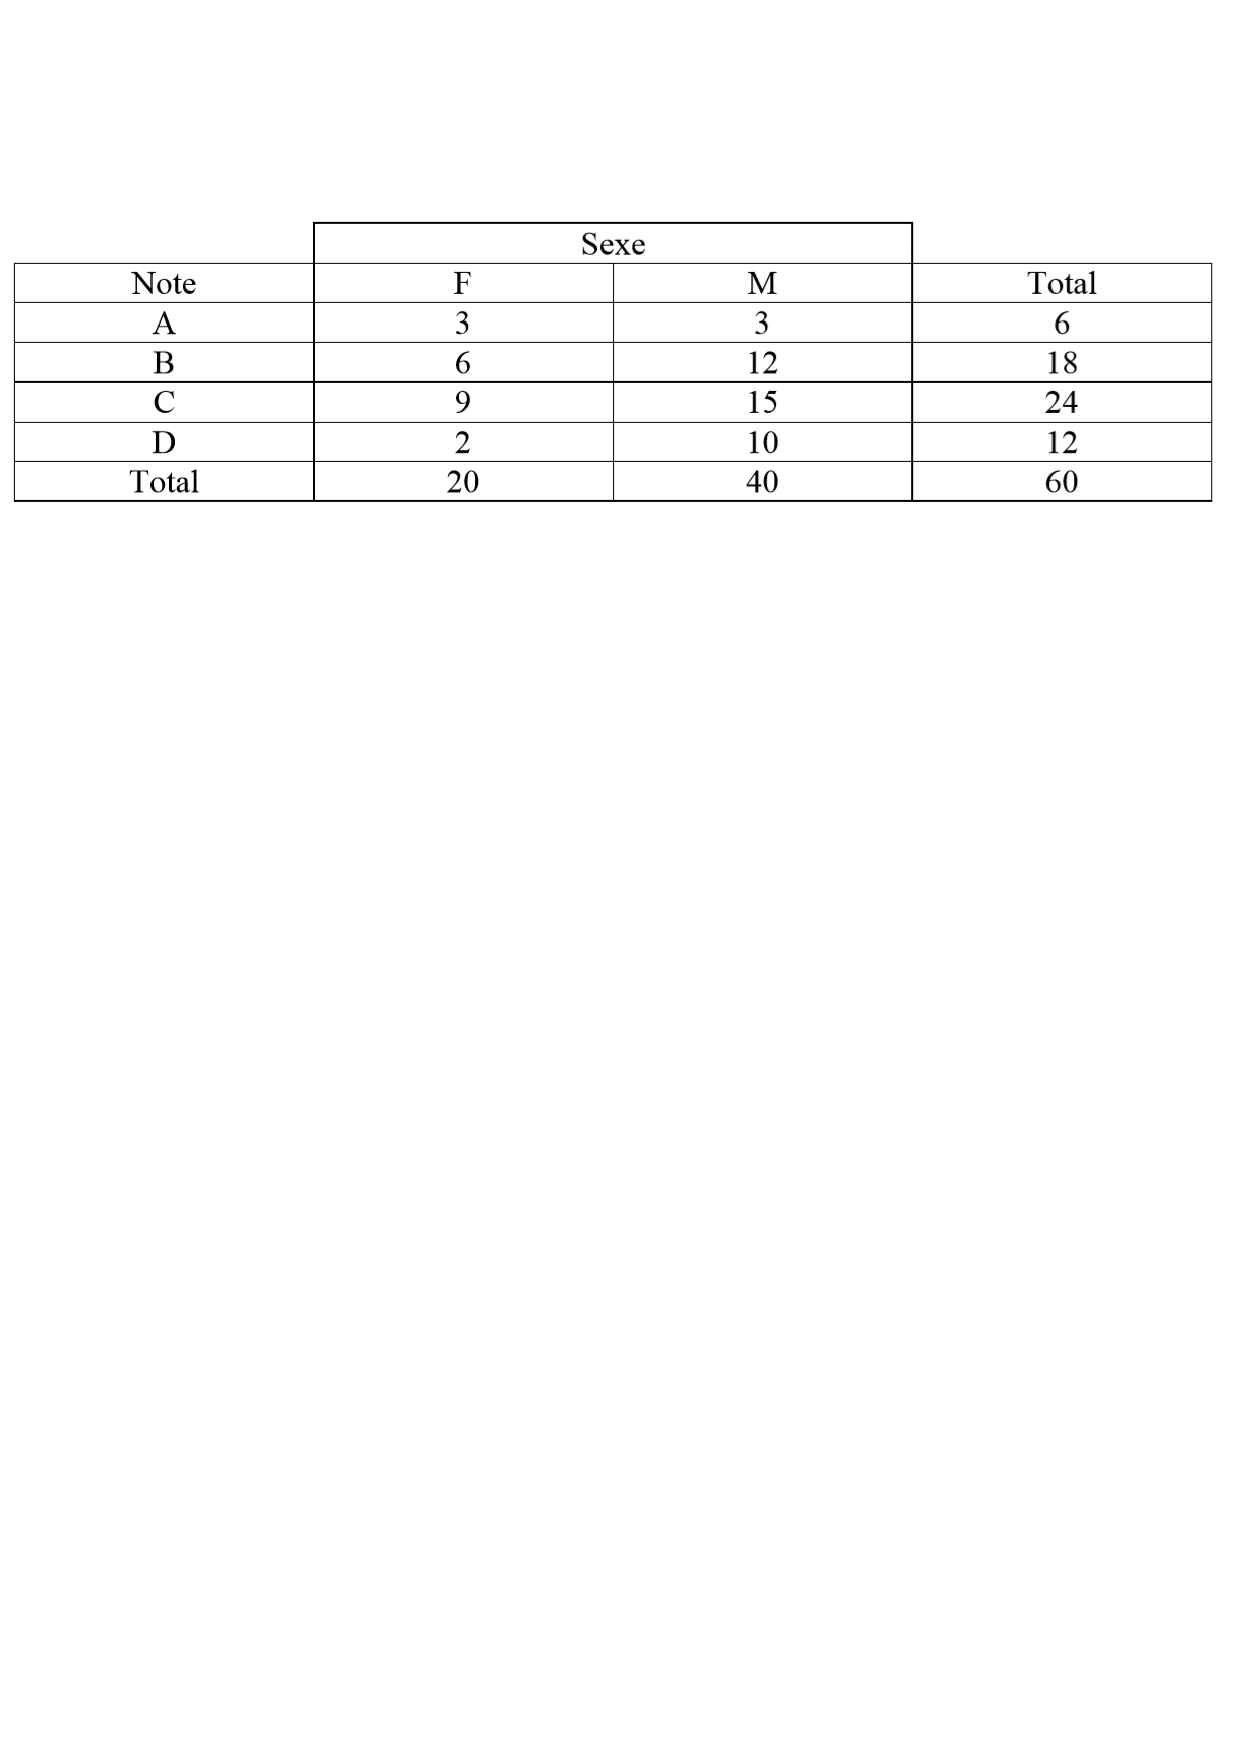
\includegraphics[width=14cm]{New579.pdf}
    \vspace{-14.3cm}
    \label{fig:New579}
  \end{center}
\end{figure}

\begin{parts}
\part Quel pourcentage d’élèves sont des femmes qui ont obtenu un D? 
\begin{solution}
\begin{eqnarray*}
\dfrac{2}{60}&=&\dfrac{1}{30}\approx 3,33 \%.
\end{eqnarray*}
\end{solution}
\part Quel pourcentage d’élèves qui ont obtenu un D sont des femmes?
\begin{solution}
\begin{eqnarray*}
\dfrac{2}{12}&=&\dfrac{1}{6}\approx 16,67 \%.
\end{eqnarray*}
\end{solution}

\part Quel pourcentage d’hommes ont obtenu un B?
\begin{solution}
\begin{eqnarray*}
\dfrac{12}{40}&=&\dfrac{3}{10}= 30,0 \%.
\end{eqnarray*}
\end{solution}

\part Quel pourcentage d’élèves sont des hommes ayant obtenu un B?
\begin{solution}
\begin{eqnarray*}
\dfrac{12}{60}&=&\dfrac{1}{5}= 20,0 \%.
\end{eqnarray*}
\end{solution}

\part Quel pourcentage d’élèves sont des femmes ayant obtenu un A ou B?
\begin{solution}
\begin{eqnarray*}
\dfrac{3+6}{60}&=&\dfrac{9}{60}=\dfrac{3}{20}= 15,0 \%.
\end{eqnarray*}
\end{solution}

\part Quel pourcentage de femmes ont obtenu un A ou B?
\begin{solution}
\begin{eqnarray*}
\dfrac{3+6}{20}&=&\dfrac{9}{20}=45,0 \%.
\end{eqnarray*}
\end{solution}
\end{parts}

\bigskip

\question Parmi les méthodes d’échantillonnage (aléatoire simple, systématique, stratifié, par grappes, à l’aveuglette, de volontaires ou par quotas), laquelle a été employée pour prélever l’échantillon?

\begin{parts}
\part Une entreprise désire savoir si l'ordinateur sur lequel un employé travaille a une influence sur son rendement au travail. L’analyste engagé par la compagnie choisit de façon arbitraire 20 \% des employés de chacun des dix départements afin d’en évaluer le rendement.
\begin{solution}
Échantillonnage par quotas.
\end{solution}

\part Dans le but de former une table ronde pour discuter de la position du gouvernement fédéral au sujet des manifestations en Afrique, un organisme prônant la paix fait appel à tous les élèves en sciences humaines. Dix-sept personnes répondent à l’appel.
\begin{solution}
Échantillonnage de volontaires.
\end{solution}

\part Une firme de sondage veut connaître les intentions de vote des électeurs montréalais. On sélectionne au hasard 50 pages du bottin téléphonique de Montréal et on appelle tous les numéros de ces pages.
\begin{solution}
Échantillonnage par grappes (les pages sont les grappes).
\end{solution}

\part Postée à l'entrée de la bibliothèque de votre collège, Antonia interroge les élèves afin de connaître leur opinion sur les nouveaux livres offerts.%GRENON À l'aveuglette
\begin{solution}
Échantillonnage à l'aveuglette.
\end{solution}


\end{parts}

\vspace{1cm}

Les pages 155 et 156 du manuel offrent un très bon résumé des définitions, mesures et interprétations importantes pour l'examen.

\newpage

\begin{center}
\underline{\textbf{\LARGE{Formules fournies à l'examen}}}
\end{center}

\vspace{1cm}

\begin{itemize}
\item $\mu=\dfrac{\sum\limits_{i=1}^{N}x_{i}}{N}$
\vspace{0.3cm}

\item $\mu=\dfrac{\sum\limits_{i=1}^{k}x_{i}n_{i}}{N}$

\vspace{0.3cm}

\item $\mu=\sum\limits_{i=1}^{k}x_{i}f_{i}$
\vspace{0.3cm}

\item $\mu=\dfrac{\sum\limits_{i=1}^{k}m_{i}n_{i}}{N}$

\vspace{0.3cm}

\item $\sigma=\sqrt{\frac{\sum\limits_{i=1}^{k}(x_{i}-\mu)^{2}n_{i}}{N}}$

\vspace{0.3cm}

\item $\sigma=\sqrt{\sum\limits_{i=1}^{k}(x_{i}-\mu)^{2}f_{i}}$

\vspace{0.3cm}

\item $\sigma=\sqrt{\frac{\sum\limits_{i=1}^{k}(m_{i}-\mu)^{2}n_{i}}{N}}$

\vspace{0.3cm}

\item $\sigma=\sqrt{\sum\limits_{i=1}^{k}(m_{i}-\mu)^{2}f_{i}}$

\vspace{0.3cm}

\item $s=\sqrt{\frac{\sum\limits_{i=1}^{k}(x_{i}-\bar{x})^{2}n_{i}}{n-1}}$

\vspace{0.3cm}

\item $s=\sqrt{\frac{\sum\limits_{i=1}^{k}(m_{i}-\bar{x})^{2}n_{i}}{n-1}}$
\end{itemize}


\end{questions}
\end{document}

